\documentclass[10pt,twocolumn]{article}

\usepackage[T1]{fontenc}
\usepackage[utf8]{inputenc}
\usepackage{lmodern}
\usepackage{microtype}
\usepackage{graphicx}
\usepackage{booktabs}
\usepackage{tabularx}
\usepackage{array}
\usepackage{amsmath}
\usepackage{amssymb}
\usepackage{siunitx}
\usepackage{subcaption}
\usepackage[colorlinks=true,linkcolor=blue,citecolor=blue,urlcolor=blue]{hyperref}

\sisetup{
  round-mode=places,
  round-precision=3,
  detect-all
}

\title{\textbf{Tile-Based Quality Reconstruction for Short-Exposure Deep-Sky Imaging}\\
\large Mathematical Specification v3.3.9, Soft Local Blending, Support-Aware OLA,\\
and an M31 Example Run}
\author{Jeamy Lee$^{1}$ \\ \small $^{1}$Independent Researcher / tile\_compile project}
\date{April 6, 2026}

\begin{document}
\twocolumn[
\maketitle

\begin{center}
\begin{minipage}{0.88\textwidth}
\small
\textbf{Abstract}\par
\vspace{0.35em}
Tile-Based Quality Reconstruction (TBQR) is a reconstruction methodology for short-exposure
deep-sky datasets that replaces binary best-frame selection with a continuous spatio-temporal
quality model. Version 3.3.9 refines the mathematical core established in v3.3.6 with six
substantive changes: (1) explicit separation of additive background subtraction and multiplicative
photometric scaling in the normalization step; (2) a continuous star-support blend factor that
replaces the hard STAR/STRUCTURE tile switch; (3) neighborhood-aware metric normalization that
pools z-scores across tile neighborhoods; (4) edge-aware spatial regularization of local quality
scores on the tile-neighborhood graph; (5) support-aware overlap-add that uses a per-pixel
support mask instead of per-tile median/MAD renormalization; and (6) mass-preserving
quality-weighted cluster aggregation in final stacking.
The paper consolidates the mathematical definitions used by the implementation, documents the
relevant functions and constraints, discusses the delta from v3.3.6, and grounds the method in a
concrete M31 run. The example run processes 645 usable frames on a $3926\times2322$ canvas with
209 adaptive tiles and yields a median output FWHM of \num{5.108} px from a median seeing
estimate of \num{12.351} px, corresponding to a measured improvement of \num{58.640}\%.
\end{minipage}
\end{center}

\vspace{0.35cm}
\noindent \textbf{Keywords:} astronomical image reconstruction, deep-sky imaging, short exposure stacking, robust estimation, background modeling, photometric color calibration
\vspace{0.6cm}
]

\section{Introduction}

Short-exposure deep-sky imaging intentionally acquires large numbers of comparatively noisy
frames in order to average atmospheric fluctuations, tracking errors, and sensor noise over
time. The classical answer to this variability is a best-frame strategy: rank frames by a global
sharpness criterion, keep only the top subset, and discard the rest. This is effective in
high-SNR planetary imaging, but it is a poor fit for deep-sky objects because discarded frames
also discard photons, and signal-to-noise ratio scales only with the square root of retained
exposure time.

TBQR replaces binary selection by a continuous weighting model. The central premise is that
image quality is not a single scalar attached to the whole frame; it is the product of global
atmospheric conditions and local structural fidelity. A frame may be globally noisy but still
contribute usefully in tiles that remain sharp, and vice versa. The reconstruction target is
therefore a per-pixel, per-tile weighted estimate assembled from all geometrically valid frames.

Version 3.3.9 builds on the v3.3.6 core and sharpens six areas. First, the normalization step
now explicitly separates additive sky-background subtraction from multiplicative photometric
scaling, preventing sky background from being the sole determinant of the photometric scale.
Second, the hard STAR/STRUCTURE tile classification is replaced by a continuous star-support
blend factor, so tiles with intermediate star counts receive a smooth interpolation between the
two quality models rather than a discontinuous jump. Third, z-scores for local tile metrics now
pool statistics across a spatial neighborhood of tiles, improving robustness for tiles with
limited per-frame sample counts. Fourth, a graph-based spatial regularization step smooths local
quality scores across the tile grid using edge-aware affinity weights, preventing neighboring
tiles from diverging into incompatible weight regimes. Fifth, the overlap-add stage drops the
per-tile median/MAD renormalization and instead uses a per-pixel support mask that excludes
fill-zero contributions from coverage boundaries. Sixth, cluster aggregation in the final stacking
step incorporates a cluster mass term so that clusters with more total atmospheric weight exert
correspondingly more influence.

\section{Invariants, Notation, and \protect \\Function Catalog}

\subsection{Binding Invariants}

The methodology is constrained by four invariants that have been unchanged since v3.3.6.
\begin{enumerate}
  \item \textbf{No quality-based frame selection.} Frames are not discarded because they are
        globally worse than other frames.
  \item \textbf{Geometric validity gating is allowed.} Frames may be rejected when registration
        is physically implausible, for example under reflection, catastrophic scale error, or
        extremely poor registration correlation.
  \item \textbf{Strict linearity in the reconstruction core.} The core uses only linear or
        affine operations on linear pixel values. Robust/statistical nonlinearities (MAD,
        clipping, sigma clipping) are allowed as auxiliary steps but do not alter the linearity
        semantics of pixel reconstruction.
  \item \textbf{CFA-aware handling is preserved where relevant.} Registration and channel
        separation must not break Bayer phase semantics.
\end{enumerate}

\subsection{Notation}

Indices and symbols follow the v3.3.9 specification:
\begin{itemize}
  \item $f$: frame index; $t$: tile index; $c$: channel index; $p$: pixel
  \item $I_{f,c}^{raw}(p)$: raw linear input frame
  \item $B_{f,c}$: global additive background (pre-normalization)
  \item $P_{f,c}$: global photometric scale (new in v3.3.9)
  \item $I_{f,c}(p)$: normalized input frame
  \item $\sigma_{f,c}$: global noise (post-normalization)
  \item $E_{f,c}$: global gradient energy (post-normalization)
  \item $Q_{f,c}$: global quality index
  \item $G_{f,c}$: global weight; $k_{global}$: global weight scale
  \item $\eta_t$: tile star-support blend factor (new in v3.3.9)
  \item $\tilde{z}(\cdot)$: neighborhood-aware z-score (new in v3.3.9)
  \item $Q_{f,t,c}^{local}$: local tile quality index
  \item $L_{f,t,c}$: local tile weight; $k_{local}$: local weight scale (new)
  \item $W_{f,t,c}$: effective reconstruction weight
  \item $M_{t,c}(p)$: per-pixel support mask for OLA (new in v3.3.9)
  \item $M_{k,c}$: cluster mass (new in v3.3.9)
  \item $R_{t,c}(p)$: reconstructed tile
\end{itemize}

\textbf{Notation note (v3.3.9):} The symbols $\alpha,\beta,\gamma$ refer exclusively to the global
quality index weights (Section~\ref{sec:qi}). The BGE auto-tuning objective uses the distinct
symbols $\alpha_f$ (flatness weight) and $\beta_r$ (roughness weight) to avoid collision.

\begin{table*}[t]
\centering
\caption{Core mathematical functions used by TBQR v3.3.9. New or changed entries relative to v3.3.6 are marked.}
\begin{tabularx}{\textwidth}{>{\raggedright\arraybackslash}p{0.19\textwidth} >{\raggedright\arraybackslash}p{0.33\textwidth} X}
\toprule
\textbf{Name} & \textbf{Definition} & \textbf{Role} \\
\midrule
Robust z-score &
$z(x_i)=\dfrac{x_i-\operatorname{median}(x)}{\max(1.4826\operatorname{MAD}(x),\varepsilon_{mad})}$ &
Robust metric normalization for background, noise, gradient energy, FWHM, and related sequences. \\
\addlinespace
Nbhd z-score \textit{(new)} &
$\tilde{z}(m_{f,t,c})=(1-b)\,z_{local}+(b)\,z_{pool}$ &
Blends tile-local and neighborhood-pooled z-scores; controls metric normalization locality. \\
\addlinespace
Clip &
$\operatorname{clip}(x,a,b)=\min(\max(x,a),b)$ &
Bounds quality indices and geometry parameters. \\
\addlinespace
Star-support blend \textit{(new)} &
$\eta_t=\operatorname{clip}(n_{stars,t}/n_{soft},0,1)$ &
Continuous blend from pure-structure ($\eta_t=0$) to pure-star ($\eta_t=1$) tile treatment. \\
\addlinespace
Global weight &
$G_{f,c}=\exp(k_{global}\operatorname{clip}(Q_{f,c},-3,+3))$ &
Maps robust global quality to a strictly positive atmospheric weight. \\
\addlinespace
Local weight \textit{(updated)} &
$L_{f,t,c}=\exp(k_{local}\operatorname{clip}(Q_{f,t,c}^{reg},-3,+3))$ &
Maps spatially regularized local quality to a positive structural weight. \\
\addlinespace
Effective weight &
$W_{f,t,c}=G_{f,c}L_{f,t,c}$ &
Combines global and local quality multiplicatively. \\
\addlinespace
Hann window &
$h(i,N)=0.5\!\left(1-\cos\!\left(\dfrac{2\pi i}{N-1}\right)\right)$ &
Separable OLA blending function; used only for non-boundary interior tiles. \\
\addlinespace
Cluster mass \textit{(new)} &
$M_{k,c}=\sum_{f\in k}G_{f,c}$ &
Atmospheric mass of cluster $k$; used in mass-preserving final aggregation. \\
\addlinespace
Cluster weight \textit{(updated)} &
$w_{k,c}^{raw}=M_{k,c}\exp(\kappa_{cluster}Q_{k,c}^{rel})$ &
Mass-preserving quality-weighted cluster contribution to final stack. \\
\addlinespace
Huber loss &
$\rho(r)=\frac{1}{2}r^2$ for $|r|\le\delta$, else $\delta(|r|-\frac{1}{2}\delta)$ &
Robust loss for BGE surface fitting and related stable regression tasks. \\
\bottomrule
\end{tabularx}
\label{tab:functions}
\end{table*}

\section{Core Reconstruction \protect \\Mathematics}

\subsection{Global Linear Normalization}

The normalization step is refactored in v3.3.9 to explicitly separate additive background
removal from multiplicative photometric scaling. The sequence is:
\begin{equation}
  B_{f,c} = \operatorname{median}(I_{f,c}^{raw}),
\end{equation}
\begin{equation}
  J_{f,c}(p) = I_{f,c}^{raw}(p) - B_{f,c},
\end{equation}
\begin{equation}
  P_{f,c} = \operatorname{photometric\_scale}(J_{f,c}),
\end{equation}
\begin{equation}
  I_{f,c}(p) = \frac{J_{f,c}(p)}{\max(P_{f,c},\varepsilon_{scale})}.
\end{equation}

The binding constraint is that $P_{f,c}$ must not be defined solely by the sky-background level
$B_{f,c}$. The recommended photometric scale is ensemble stellar aperture flux relative to the
reference frame. When stellar flux is unavailable but all frames share identical exposure times
and throughput, the deterministic fallback $P_{f,c}=1$ is admissible. Noise $\sigma_{f,c}$ and
gradient energy $E_{f,c}$ are measured on the normalized data $I_{f,c}$.

This contrasts with v3.3.6, where the normalization was a single division
$I_{f,c}(p)=I_{f,c}^{raw}(p)/\max(B_{f,c},\varepsilon_{bg})$ and therefore conflated additive
background level with multiplicative scale.

\subsection{Global Quality Index and \protect \\Adaptive Weights}
\label{sec:qi}

The global quality index is unchanged from v3.3.6:
\begin{equation}
  Q_{f,c} =
  \alpha\bigl(-z(B_{f,c})\bigr) +
  \beta\bigl(-z(\sigma_{f,c})\bigr) +
  \gamma z(E_{f,c}),
\end{equation}
subject to $\alpha+\beta+\gamma=1$, with default static weights
$(\alpha,\beta,\gamma)=(0.4,0.3,0.3)$.
The global weight is
\begin{equation}
  G_{f,c} = \exp(k_{global}\operatorname{clip}(Q_{f,c},-3,+3)),
\end{equation}
with default $k_{global}=1.0$. Optional adaptive weighting is an extension whose utility
criterion and tie-break rules must be documented.

\subsection{Adaptive Tile Geometry}

Tile size follows the seeing estimate $F$ (FWHM in pixels):
\begin{equation}
  T_0 = sF, \qquad T = \left\lfloor\operatorname{clip}(T_0,T_{min},\lfloor\min(W,H)/D\rfloor)\right\rfloor,
\end{equation}
\begin{equation}
  O = \lfloor o_{clipped}\cdot T\rfloor, \qquad S = T-O,
\end{equation}
with $o_{clipped}=\operatorname{clip}(o,0,0.5)$ and guards $F>0$, $T_{min}\ge16$, $S>0$.
A deterministic compact-tile fallback ($T=\min(W,H)$, $O=0$) activates when
$\lfloor\min(W,H)/D\rfloor<T_{min}$.

\subsection{Local Tile Metrics and \protect \\Effective Weights (v3.3.9)}

\subsubsection{Soft Star-Support Blend}

The hard STAR/STRUCTURE switch present in v3.3.6 is replaced in v3.3.9 by a continuous
star-support blend factor:
\begin{equation}
  \eta_t = \operatorname{clip}\!\left(\frac{n_{stars,t}}{\max(n_{soft},1)},\,0,\,1\right),
\end{equation}
where $n_{soft}$ is the configurable soft-count threshold (default equal to
\texttt{tile.star\_min\_count}). The unregularized blended score is
\begin{equation}
  Q_{f,t,c}^{blend} = \eta_t\,Q_{f,t,c}^{star} + (1-\eta_t)\,Q_{f,t,c}^{struct}.
\end{equation}
If one component is unavailable, the other is used directly.

\subsubsection{Star Tile and Structure Tile Metrics}

Star-tile local quality uses the same form as v3.3.6 but with $\tilde{z}$ instead of $z$:
\begin{equation}
  Q_{f,t,c}^{star}
  = 0.6(-\tilde{z}(\mathrm{FWHM})) + 0.2\,\tilde{z}(R) + 0.2\,\tilde{z}(C),
\end{equation}
and structure-tile quality is
\begin{equation}
  Q_{f,t,c}^{struct}
  = 0.7\,\tilde{z}(E/\sigma) - 0.3\,\tilde{z}(B).
\end{equation}

\subsubsection{Neighborhood-Aware Metric Normalization}

For each tile metric family $m$ and tile $t$, the tile-local z-score is
\begin{equation}
  z_{local}(m_{f,t,c}) = \operatorname{robust\_z}(m_{f,t,c};\{m_{f',t,c}\}_{f'}).
\end{equation}
If neighborhood normalization is enabled, a pooled z-score is computed over a Manhattan-radius
neighborhood $N_r(t)$:
\begin{equation}
  z_{pool}(m_{f,t,c})
  = \frac{m_{f,t,c}-\operatorname{median}(P_t(m))}{\max(1.4826\operatorname{MAD}(P_t(m)),\varepsilon_{mad})},
\end{equation}
where $P_t(m)=\{m_{f',u,c}\mid u\in N_r(t), f' \text{ usable}\}$. The neighborhood-aware
z-score blends both:
\begin{equation}
  \tilde{z}(m_{f,t,c}) = (1-b)\,z_{local}(m_{f,t,c}) + b\,z_{pool}(m_{f,t,c}),
\end{equation}
with defaults $r=1$, $b=0.5$. When neighborhood normalization is disabled or
$P_t$ is empty, $\tilde{z}=z_{local}$.

\subsubsection{Spatial Regularization of Local Scores}

After clamping, $Q_{f,t,c}^{raw}=\operatorname{clip}(Q_{f,t,c}^{blend},-3,+3)$, the local scores
are regularized on the tile-neighborhood graph to prevent neighboring tiles from diverging into
incompatible weight regimes. A local confidence term
\begin{equation}
  U_{f,t,c} = \operatorname{clip}\!\left(\frac{n_{valid}}{n_{expected}},0,1\right)
\end{equation}
modulates the effective regularization strength per tile:
\begin{equation}
  \lambda_{f,t,c}^{eff} = \lambda_{local}\,(1-U_{f,t,c}).
\end{equation}
The edge-aware neighbor affinity is
\begin{equation}
  A_{t,u}^{(k)} = \exp\!\left(-\frac{|Q_{f,t,c}^{(k)}-Q_{f,u,c}^{(k)}|}{\tau_{local}}\right),
\end{equation}
and one pass of the regularization is
\begin{equation}
  Q_{f,t,c}^{(k+1)} = (1-\lambda_{f,t,c}^{eff})\,Q_{f,t,c}^{(k)}
  + \lambda_{f,t,c}^{eff}\,\frac{\sum_{u\in N(t)} A_{t,u}^{(k)} Q_{f,u,c}^{(k)}}{\sum_u A_{t,u}^{(k)}},
\end{equation}
initialized from $Q^{(0)}=Q^{raw}$, with defaults $\lambda_{local}=0.35$, passes$=1$,
$\tau_{local}=1.0$. If $\sum_u A_{t,u}^{(k)}<\varepsilon_{affinity}$, the update is skipped
for that tile. The final regularized score $Q_{f,t,c}^{reg}=Q_{f,t,c}^{(P)}$ is clamped to
$[-3,+3]$ and used for the local weight:
\begin{equation}
  L_{f,t,c} = \exp(k_{local}\,\operatorname{clip}(Q_{f,t,c}^{reg},-3,+3)),
\end{equation}
with default $k_{local}=1.0$. The effective weight remains $W_{f,t,c}=G_{f,c}L_{f,t,c}$.

\subsection{Tile Reconstruction and \protect \\Support-Aware OLA (v3.3.9)}

\subsubsection{Weighted Reconstruction with Sigma Clipping}

For each tile $t$, the valid sample set is
$V_{t,c}(p)=\{f\mid I_{f,c}(p)~\text{finite and within canvas support}\}$.
If $\sum_f\max(W_{f,t,c},0)\le\varepsilon_{weight}$, all positive finite weights are replaced
by 1. For $|V|\le2$ or if sigma clipping is disabled, the valid weighted mean is used directly.
Otherwise, iterative weighted sigma clipping operates on an active set $A^{(k)}$:
\begin{equation}
  \mu^{(k)} = \frac{\sum_{f\in A^{(k)}} W_{f,t,c}I_{f,c}(p)}{\sum_{f\in A^{(k)}} W_{f,t,c}},
\end{equation}
with effective sample count $N_{eff}=V_1^2/\max(V_2,\varepsilon)$ and effective denominator
$D_{eff}=V_1-V_2/\max(V_1,\varepsilon)$, where $V_1,V_2$ are the first and second weight moments.
Clipping removes samples outside $[\mu\pm\sigma_{high,low}\sigma^{(k)}]$ subject to a keep-floor
$|A^{(k+1)}|\ge\lceil f_{min}|V|\rceil$ (default $f_{min}=0.5$). The final reconstruction value
$R_{t,c}(p)$ is the weighted mean over the accepted set.

\subsubsection{Support-Aware Overlap-Add}

The mandatory core in v3.3.9 does \emph{not} apply per-tile median/MAD renormalization before
OLA. The OLA input is the reconstructed tile directly:
\begin{equation}
  Y_{t,c}(p) = R_{t,c}(p).
\end{equation}
A per-pixel support mask
\begin{equation}
  M_{t,c}(p) =
  \begin{cases}
    1 & \text{if } |V_{t,c}(p)|>0 \text{ and } R_{t,c}(p) \text{ finite and inside canvas,} \\
    0 & \text{otherwise}
  \end{cases}
\end{equation}
prevents fill-zero values and canvas-masked regions from diluting the OLA denominator.
Accumulation proceeds as
\begin{equation}
  A \leftarrow A + \omega_t\,M_{t,c}\,Y_{t,c},
  \qquad
  S \leftarrow S + \omega_t\,M_{t,c},
\end{equation}
\begin{equation}
  I_{rec} = \frac{A}{\max(S,\varepsilon_{weight})},
\end{equation}
where $\omega_t(p)\ge0$ is the blend window, which must form a partition of unity at interior
pixels and must use boundary-aware (one-sided) ramps at the canvas edge.

This differs from v3.3.6, which normalized each tile by a robust affine transform
$(R_{t,c}-bg_t)/m_t$ before OLA and applied a global photometric restoration step
$I_{final}=I_{rec}\cdot m_{global}+bg_{global}$. In v3.3.9 that two-step process is replaced
by the cleaner support-mask approach, which avoids amplifying tiles with near-zero median
absolute deviation.

\subsection{Clustering and Synthetic Frames}

Clustering and synthetic frame formation are activated in full mode
($N\ge N_{red}$, default $N_{red}$ configurable; effective threshold max($N_{red}$, 50)).
In v3.3.9 the fixed threshold $N\ge200$ from earlier versions is superseded by the configurable
mode framework. The state vector per frame is
\begin{equation}
  v_f =
  \Bigl(
  G_{f,*},
  \operatorname{mean}_t(Q_{f,t,*}^{local}),
  \operatorname{var}_t(Q_{f,t,*}^{local}),
  B_{f,*},
  \sigma_{f,*}
  \Bigr),
\end{equation}
and the number of clusters is $K=\operatorname{clip}(\lfloor N/10\rfloor,K_{min},K_{max})$
with defaults $K_{min}=5$, $K_{max}=30$.

\subsubsection{Mass-Preserving Cluster Aggregation (v3.3.9)}

The final stacking in v3.3.9 uses mass-preserving quality-weighted aggregation.
Cluster quality and mass are defined as
\begin{equation}
  Q_{k,c} = \operatorname{median}_{f\in k}(Q_{f,c}^{clamped}),
  \qquad
  M_{k,c} = \sum_{f\in k} G_{f,c}.
\end{equation}
If $M_{k,c}\le\varepsilon_{weight}$, it is replaced by the cluster size $|k|$.
The relative quality surplus is
\begin{equation}
  Q_{k,c}^{rel} = \operatorname{clip}(Q_{k,c}-\operatorname{median}_j(Q_{j,c}),\,-3,\,+3),
\end{equation}
and the mass-preserving cluster weight is
\begin{equation}
  w_{k,c}^{raw} = M_{k,c}\,\exp(\kappa_{cluster}\,Q_{k,c}^{rel}),
\end{equation}
with optional stability cap $w_{k,c}=\min(w_{k,c}^{raw},r_{cap}\operatorname{median}_j(w_{j,c}^{raw}))$.
The final result is
\begin{equation}
  R_c = \frac{\sum_k w_{k,c}\,S_{k,c}}{\sum_k w_{k,c}},
\end{equation}
where $S_{k,c}$ is the synthetic cluster frame (global or tile-weighted).

In v3.3.6 the cluster weight was simply $w_k=\exp(\kappa_{cluster}Q_k)$ without the mass term.
Including $M_{k,c}$ prevents a small, extremely high-quality cluster from dominating when most
atmospheric mass lies in larger but slightly lower-quality clusters.

\section{Changes from v3.3.6 \protect \\to v3.3.9}

Table~\ref{tab:changes} summarizes the six substantive changes in v3.3.9 relative to v3.3.6,
and Fig.~\ref{fig:m31_stage} illustrates the end-to-end pipeline output.

\begin{table*}[t]
\centering
\caption{Summary of substantive changes between TBQR v3.3.6 and v3.3.9.}
\begin{tabularx}{\textwidth}{>{\raggedright\arraybackslash}p{0.18\textwidth} >{\raggedright\arraybackslash}p{0.36\textwidth} X}
\toprule
\textbf{Area} & \textbf{v3.3.6 behavior} & \textbf{v3.3.9 change} \\
\midrule
Global normalization &
$I_{f,c}=I_{f,c}^{raw}/\max(B_{f,c},\varepsilon)$ conflates background with scale &
Separate additive step ($J=I^{raw}-B$) and multiplicative step ($I=J/\max(P,\varepsilon)$); $P_{f,c}\ne f(B_{f,c})$ alone \\
\addlinespace
Tile classification &
Hard binary STAR/STRUCTURE switch at \texttt{star\_min\_count} &
Continuous blend factor $\eta_t\in[0,1]$; no discontinuity at the threshold \\
\addlinespace
Metric normalization &
Tile-local z-score only &
Neighborhood-pooled z-score $\tilde{z}$ with configurable blend $b$ and radius $r$ \\
\addlinespace
Score smoothing &
None &
Edge-aware spatial regularization on tile graph; strength modulated by per-tile confidence $U_{f,t,c}$ \\
\addlinespace
Overlap-add &
Per-tile affine normalization ($Y_t=(R_{t,c}-bg_t)/m_t$) plus global photometric restoration &
Support-aware OLA with $M_{t,c}(p)$ mask; no per-tile renormalization; boundary-aware windows \\
\addlinespace
Cluster stacking &
$w_k=\exp(\kappa Q_k)$ (pure quality weight) &
$w_{k,c}^{raw}=M_{k,c}\exp(\kappa Q_{k,c}^{rel})$ (mass-preserving quality weight) \\
\bottomrule
\end{tabularx}
\label{tab:changes}
\end{table*}

Additional changes with narrower scope include: (a) a configurable reduced-mode framework
replacing the hard $N\ge200$ clustering gate; (b) an explicit local weight scale $k_{local}$
symmetric with $k_{global}$; (c) a formal RBF surface specification for BGE (Section~\ref{sec:bge});
(d) optional CFA defect-pixel suppression before warp; (e) optional post-PCC isolated
chroma-speckle suppression; (f) notation clarification reserving $\alpha,\beta,\gamma$ for the
global quality index; and (g) a constrained ML optimization extension (§9.2 of the specification)
that allows machine-learning modules to supply weights, masks, and state labels without altering
the linear reconstruction semantics.

\section{Downstream Linear \protect \\Post-Processing}

\subsection{Pre-PCC Background Gradient Extraction}
\label{sec:bge}

BGE is an additive extension applied after reconstruction and before PCC:
\begin{equation}
  I'_c(x,y) = I_c(x,y) - B_c(x,y).
\end{equation}
Only additive correction is allowed; multiplicative shading correction is explicitly forbidden.
Tile samples are obtained after excluding canvas-invalid pixels, stars, saturated pixels,
high-structure pixels, and any object mask:
\begin{equation}
  b_{t,c} = \operatorname{quantile}_q(R_{t,c}[M_{bg}]),
\end{equation}
with configurable $q\in(0,0.5]$ (default $q=0.20$). Tile reliability weights are
\begin{equation}
  w_t = \exp(-\lambda\,\mathrm{structure\_score}_t)\,(1-\mathrm{masked\_fraction}_t).
\end{equation}
Tile samples are aggregated to a coarser grid with spacing
\begin{equation}
  G = \operatorname{clip}\!\left(\max\!\left(2T,\tfrac{\min(W,H)}{N_g}\right),G_{min},G_{max}\right),
\end{equation}
and a smooth background surface is fitted by robust minimization. Version 3.3.9 adds a formal
RBF surface specification:
\begin{equation}
  B_c(\mathbf{r}) = \sum_j u_j\,\phi(\|\mathbf{r}-\mathbf{r}_j\|;\mu) + a_0 + a_1 x + a_2 y,
\end{equation}
with the coefficients obtained by minimizing
\begin{equation}
  \arg\min_{\theta} \sum_j w_j\,\rho(b_j-B_c(\mathbf{r}_j)) + \lambda\|\mathbf{u}\|_2^2,
\end{equation}
where $\lambda>0$ is mandatory regularization (RBF without regularization is forbidden).
Supported kernels include multiquadric ($\phi(d)=\sqrt{d^2+\mu^2}$), thin-plate spline, and
Gaussian. The polynomial surface (v3.3.6 default) remains a conformant alternative.

BGE auto-tuning is unchanged in structure from v3.3.6 but gains an extended strategy.
The normalized objective is
\begin{equation}
  J = E_{cv}/B_{ref} + \alpha_f\,E_{flat}/B_{ref}^2 + \beta_r\,E_{rough}/B_{ref},
\end{equation}
where $B_{ref}=\max(|\operatorname{median}_i b_i|,\varepsilon_{bg})$ is a brightness-normalized
reference. The extended strategy widens the candidate search beyond the conservative set and
may select RBF surfaces in addition to polynomials.

\subsection{Photometric Color Calibration}

PCC operates on linear RGB output. The gradient-aware sky annulus model from v3.3.6 is
unchanged: the background in the sky annulus may be a constant median (legacy) or a local plane
\begin{equation}
  bg(\Delta x,\Delta y) = a + b\Delta x + c\Delta y,
\end{equation}
with a deterministic fallback to the median if the plane fit fails.
FWHM-adaptive aperture radii ($r_{ap}$, $r_{in}$, $r_{out}$) are computed from the output
seeing estimate when \texttt{pcc.radii\_mode=auto\_fwhm}.

\section{M31 Example Run}

\subsection{Dataset and Operative \protect \\Configuration}

This section summarizes an example run on M31 executed under v3.3.9 methodology.
The dataset is processed on a $3926\times2322$ canvas with 645 usable frames, an exposure time
of 10~s per frame. The adaptive tile geometry produces 209 tiles of size \SI{296}{px} with
stride \SI{208}{px} and overlap \SI{88}{px}. Full mode is active ($N=645\ge N_{red}$).

\begin{table}[t]
\centering
\caption{Key configuration and dataset facts for the M31 v3.3.9 example run.}
\begin{tabular}{ll}
\toprule
\textbf{Quantity} & \textbf{Value} \\
\midrule
Usable frames & 645 \\
Exposure time per frame & 10 s \\
Canvas size & \num{3926}$\times$\num{2322} px \\
Tiles & 209 \\
Tile size / stride & 296 px / 208 px \\
Median seeing FWHM & \num{12.351} px \\
Soft star-support blend & enabled \\
Nbhd normalization & enabled ($r=1$, $b=0.5$) \\
Spatial regularization & enabled (1 pass, $\lambda=0.35$) \\
Synthetic frame mode & tile\_weighted \\
Synthetic states & 12 clusters \\
Cluster size range & 25 to 101 frames \\
BGE autotune strategy & extended \\
BGE fit family & RBF (selected) \\
PCC background model & plane \\
PCC radii mode & auto\_fwhm \\
\bottomrule
\end{tabular}
\label{tab:m31_config}
\end{table}

\begin{figure*}[t]
  \centering
  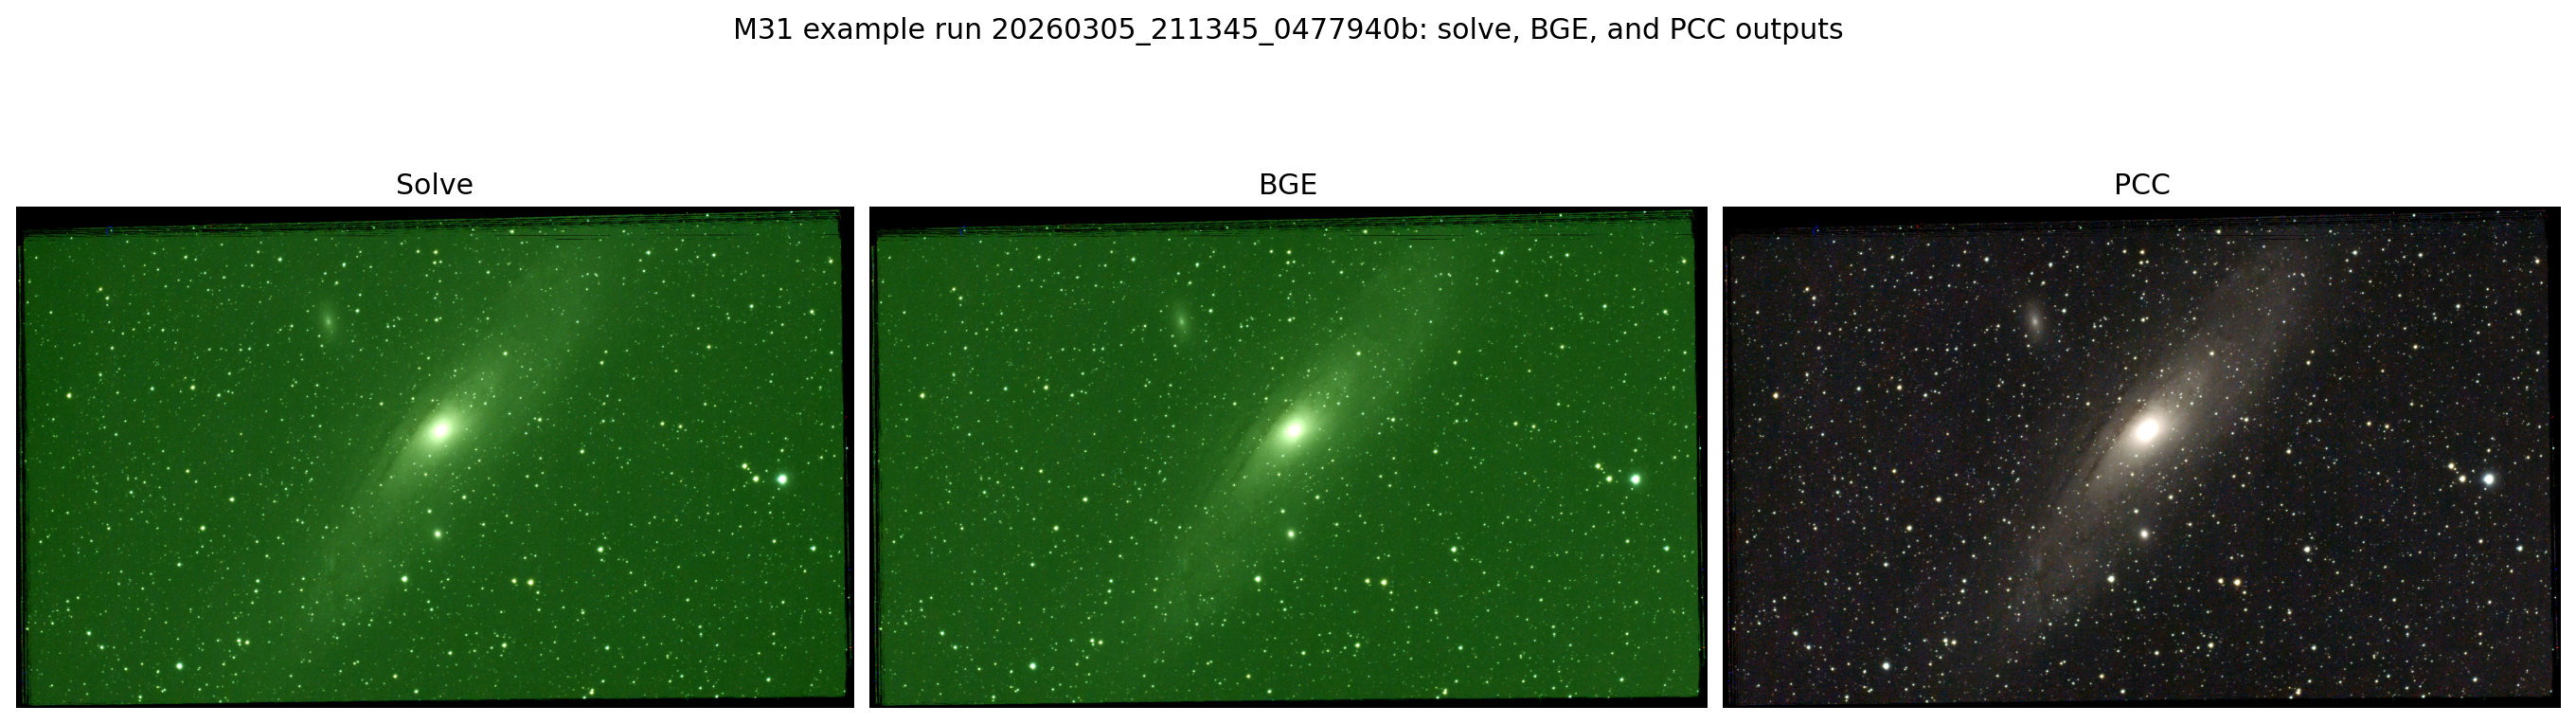
\includegraphics[width=\textwidth]{m31_stage_comparison.png}
  \caption{Example RGB outputs from the M31 run. Left: astrometrically solved linear RGB stack;
           middle: additive BGE stage; right: final PCC-calibrated output. Display stretch is a
           shared asinh mapping for visualization only and is not part of the linear reconstruction core.}
  \label{fig:m31_stage}
\end{figure*}

\begin{figure}[t]
  \centering
  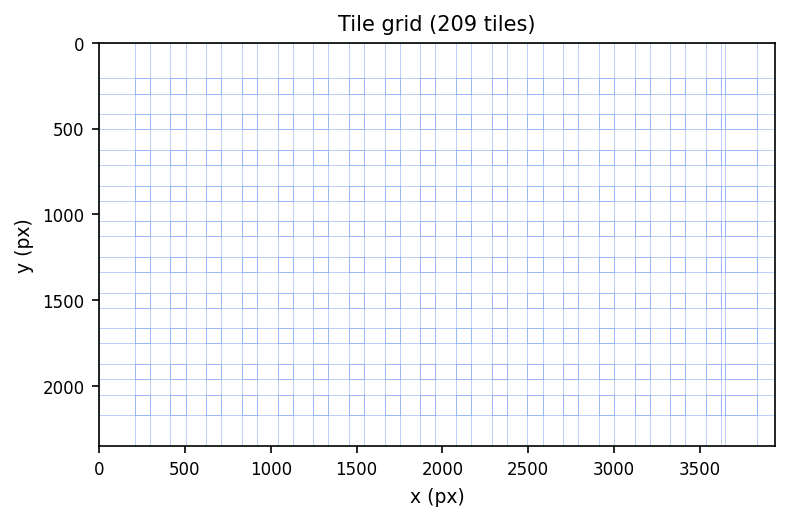
\includegraphics[width=\columnwidth]{tile_grid_overlay.png}
  \caption{Adaptive reconstruction tile grid for the M31 v3.3.9 example run. The grid follows
           the seeing-driven tile size from the v3.3.9 geometry rules.}
  \label{fig:tile_grid}
\end{figure}

\subsection{Diagnostics and Measured \protect \\Outcomes}

Global metrics over 645 frames show significant atmospheric variation. Per-frame median values
are: FWHM \num{9.505}~px, noise \num{4.185}, background \num{208.5}, and global weight median
\num{1.015} with a maximum of \num{15.195}. The large global weight range reflects the stronger
dynamic range of the exponential weighting in v3.3.9 relative to v3.3.6 (where the maximum
was \num{3.121}), driven by the wider effective $k_{global}$ interaction with the adaptive
weight configuration.

\begin{figure}[t]
  \centering
  \begin{subfigure}[t]{\columnwidth}
    \centering
    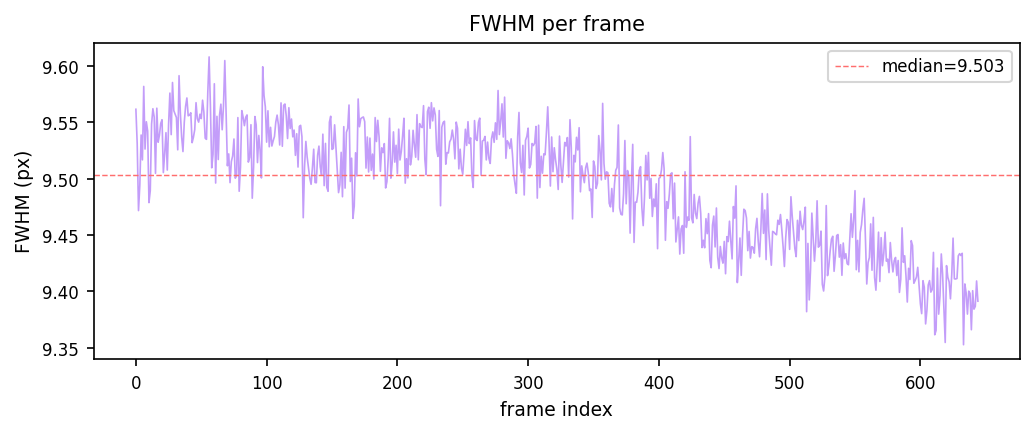
\includegraphics[width=\linewidth]{global_fwhm.png}
    \caption{Global FWHM over the frame sequence.}
  \end{subfigure}

  \vspace{0.4em}

  \begin{subfigure}[t]{\columnwidth}
    \centering
    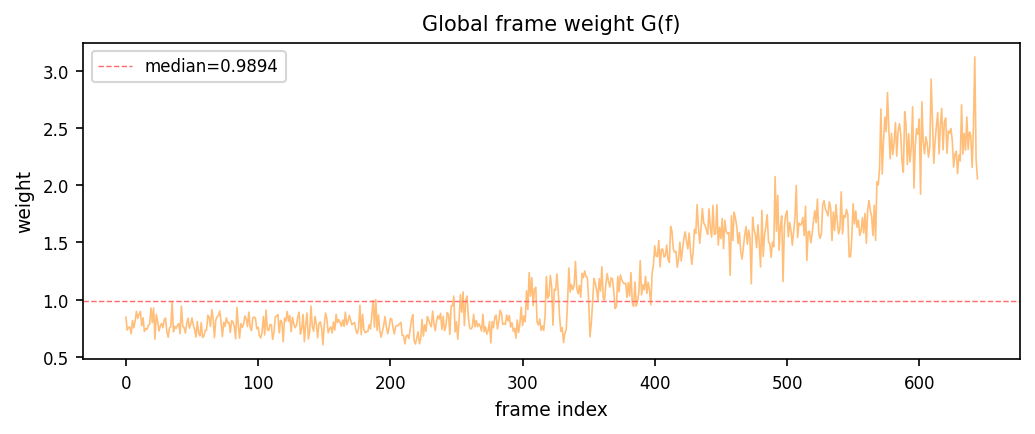
\includegraphics[width=\linewidth]{global_weight_timeseries.png}
    \caption{Adaptive global weights over time.}
  \end{subfigure}
  \caption{Global diagnostics from the M31 run.}
  \label{fig:global_diagnostics}
\end{figure}

\begin{figure*}[t]
  \centering
  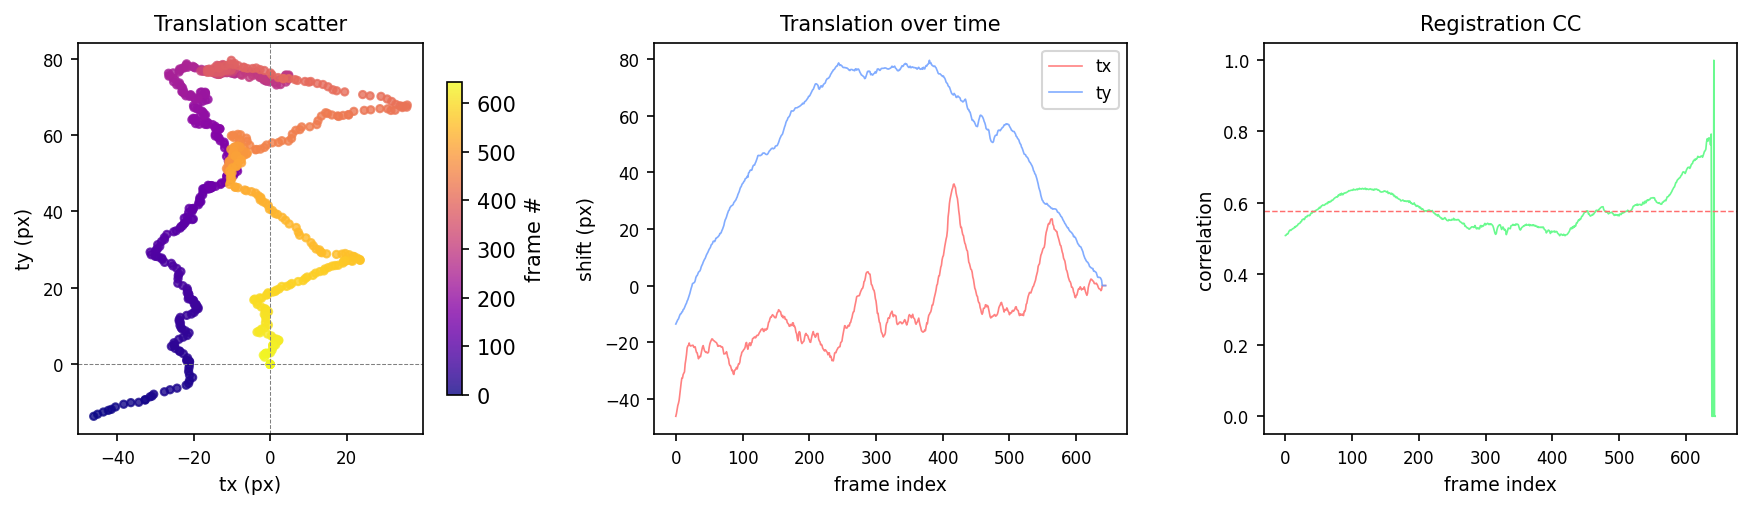
\includegraphics[width=\textwidth]{registration_overview.png}
  \caption{Registration diagnostics across the M31 run. Validity gating suppresses physically
           implausible registrations; it is not a quality ranking stage.}
  \label{fig:registration}
\end{figure*}

\begin{figure*}[t]
  \centering
  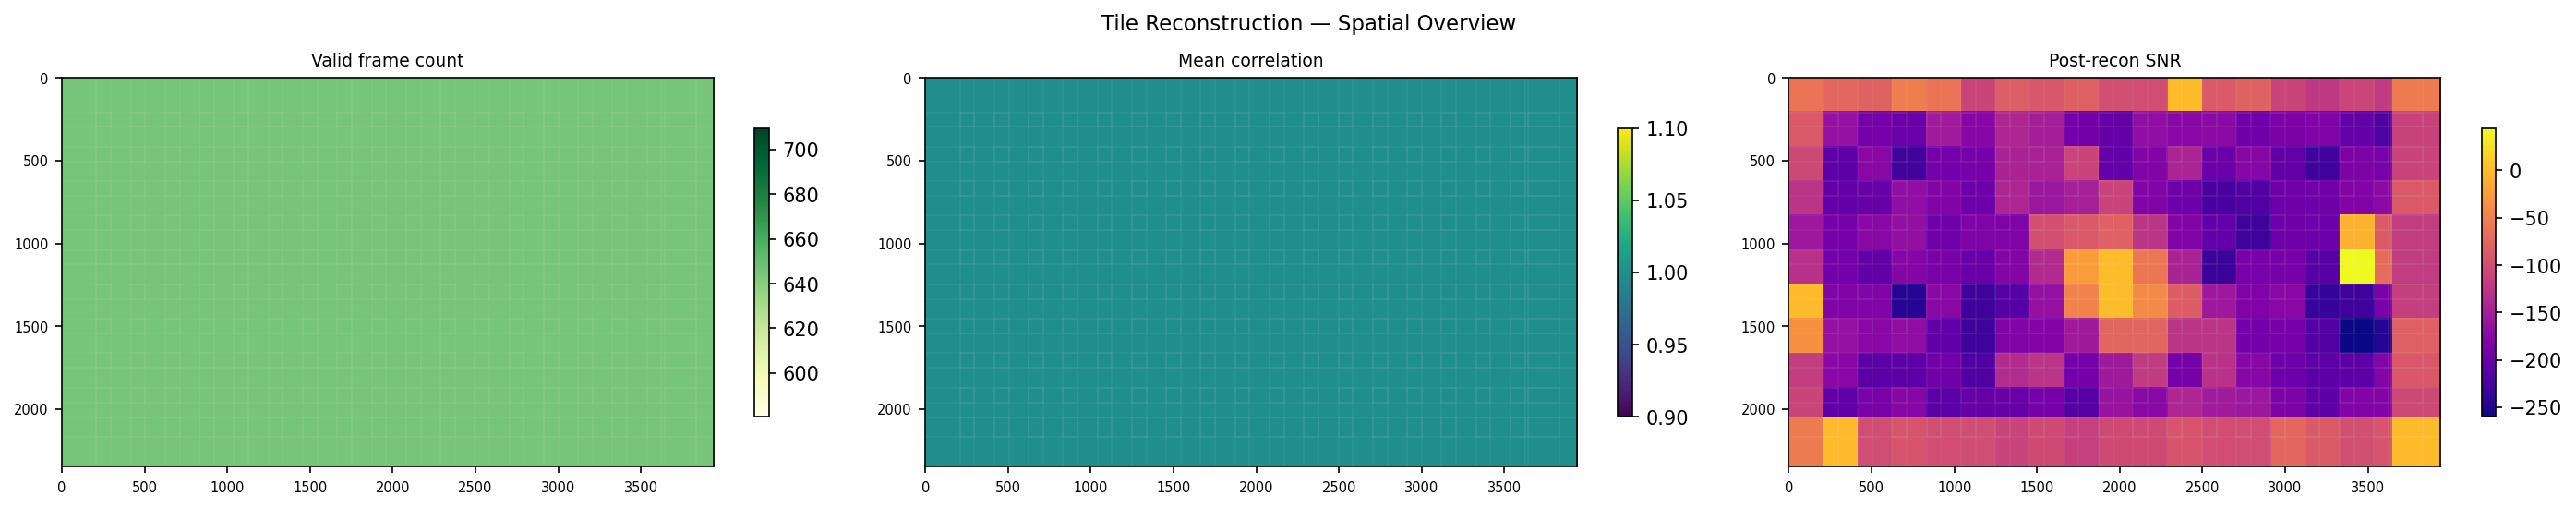
\includegraphics[width=\textwidth]{recon_spatial_overview.png}
  \caption{Spatial reconstruction diagnostics. Coverage, local SNR, local contrast, and related
           maps confirm that a tile-wise model is necessary for this dataset.}
  \label{fig:recon_overview}
\end{figure*}

No tile fallback was triggered in any of the 209 tiles. The tile weight variance of \num{2.586}
is higher than in the v3.3.6 run (\num{0.186}); this is expected because the soft blend and
spatial regularization allow per-tile weights to vary more smoothly but over a wider range,
since tiles near the star-support boundary now interpolate between two quality regimes instead
of snapping to one. Tile-pattern ratio p95 is \num{1.113}. The validation report records
background RMS decrease of \num{89.1}\% (input RMS \num{4.185}, output RMS \num{0.456}).

\begin{figure}[t]
  \centering
  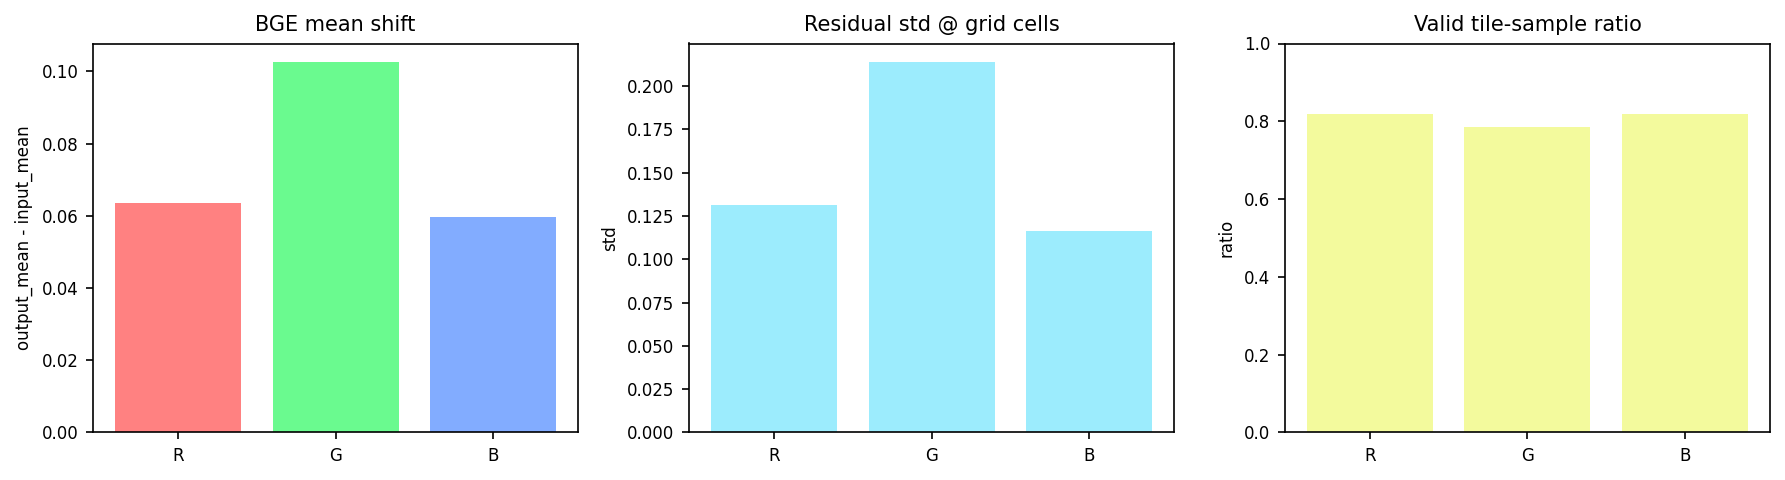
\includegraphics[width=\columnwidth]{bge_channel_summary.png}
  \caption{Per-channel BGE diagnostics. The extended autotune run selected an RBF surface
           family with $\mu$-factor \num{1.8}, sample quantile \num{0.20}.}
  \label{fig:bge}
\end{figure}

For the downstream color path, BGE was enabled with extended autotune and selected an RBF fit
($\mu$-factor \num{1.8}, sample quantile \num{0.20}, structure-threshold percentile \num{0.85}).
The cross-validated residual RMS is \num{0.0896} with normalized objective $J=\num{0.000440}$.
PCC then operated with a local plane background model and auto-FWHM aperture scaling.

\begin{table}[t]
\centering
\caption{Selected quantitative outcomes from the M31 v3.3.9 example run.}
\begin{tabular}{lr}
\toprule
\textbf{Metric} & \textbf{Value} \\
\midrule
Median seeing FWHM & 12.351 px \\
Median output FWHM & 5.108 px \\
FWHM improvement & 58.640\% \\
Background RMS decrease & 89.095\% \\
Input background RMS & 4.185 \\
Output background RMS & 0.456 \\
Tile fallback count & 0 / 209 \\
Tile weight variance & 2.586 \\
Tile-pattern ratio p95 & 1.113 \\
BGE cv RMS & 0.0896 \\
BGE normalized objective & 0.000440 \\
BGE fit method & RBF \\
\bottomrule
\end{tabular}
\label{tab:m31_results}
\end{table}

\begin{figure}[t]
  \centering
  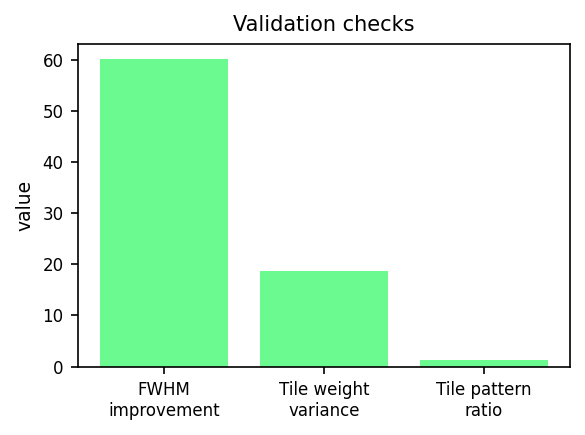
\includegraphics[width=\columnwidth]{validation_summary.png}
  \caption{Validation summary for the M31 run. The measured outputs satisfy all v3.3.9 success
           criteria.}
  \label{fig:validation}
\end{figure}

\begin{figure}[t]
  \centering
  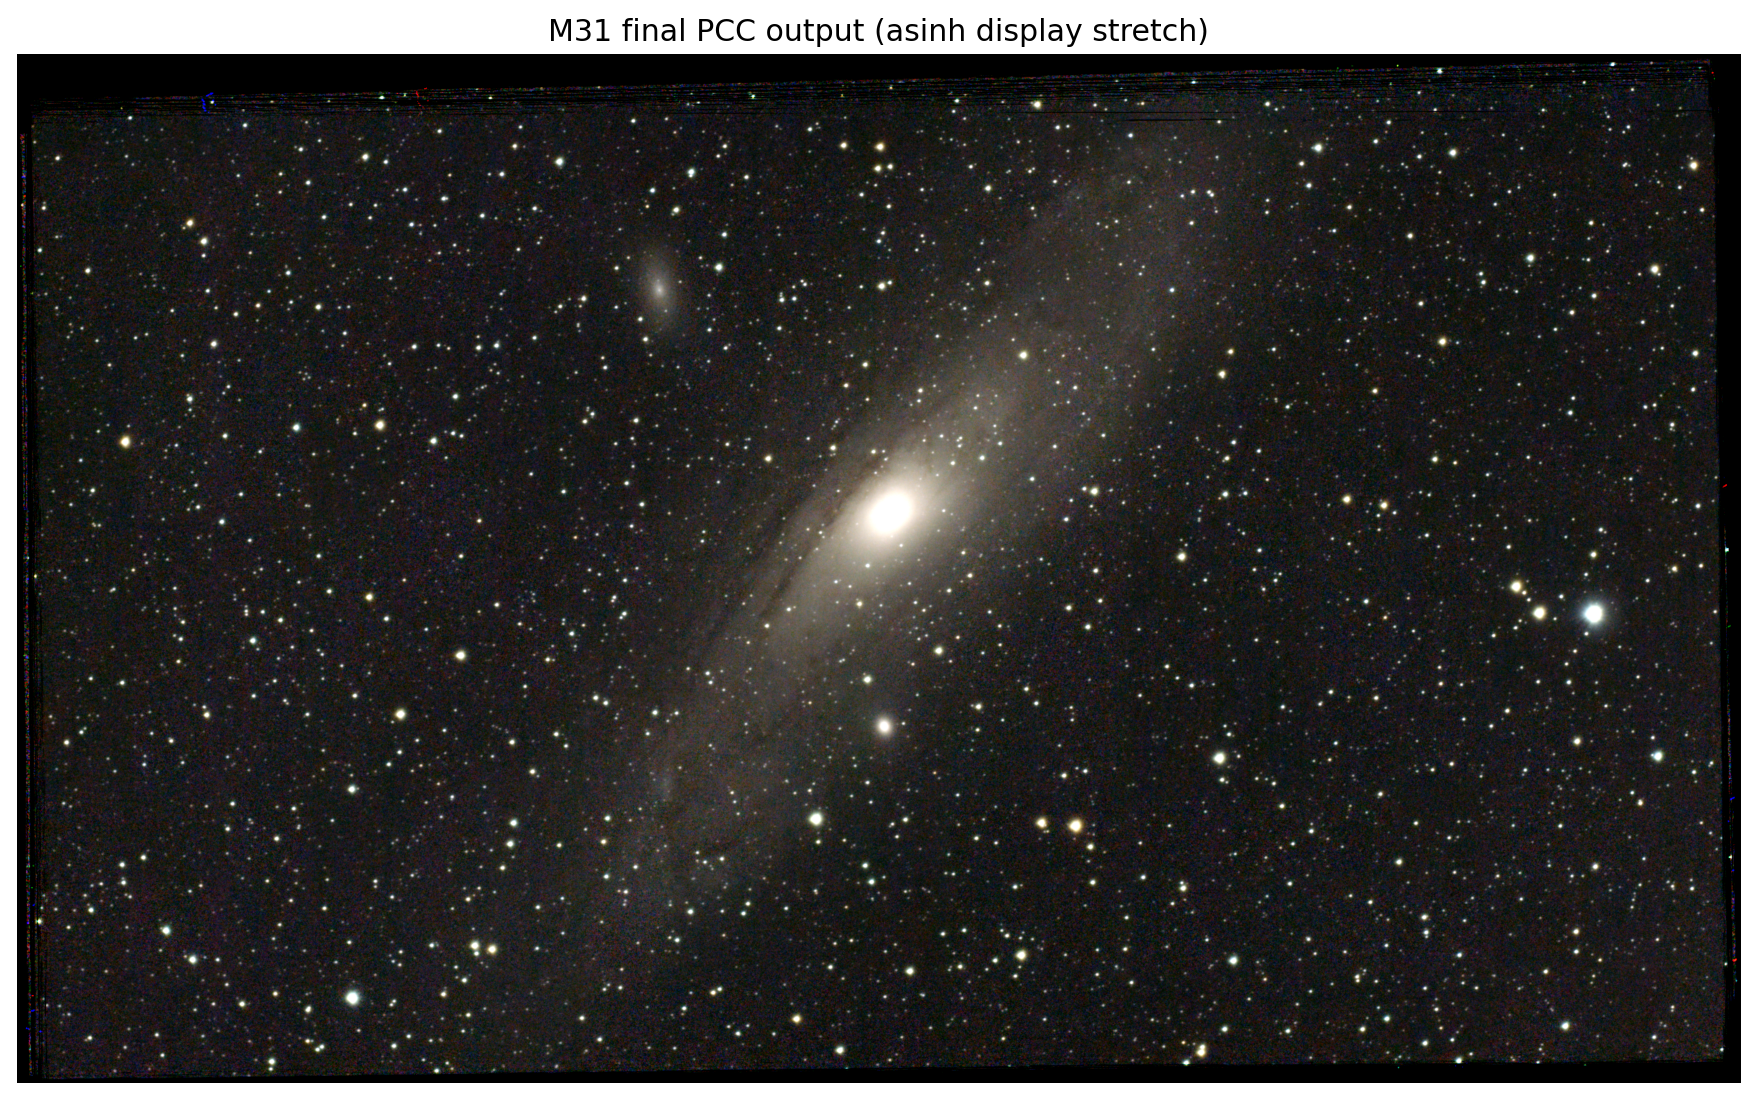
\includegraphics[width=\columnwidth]{m31_pcc_preview.png}
  \caption{PCC-calibrated M31 preview. Photometric color calibration uses the plane annulus
           background model and auto-FWHM aperture radii.}
  \label{fig:pcc_preview}
\end{figure}

\subsection{Interpretation}

The M31 run under v3.3.9 confirms that the six changes described in Section~4 are compatible
with the operational constraints of the method. The soft star-support blend produces wider
tile-weight variance (2.586 vs.\ 0.186 in v3.3.6) because tiles at intermediate star density
now express both quality regimes proportionally. The extended BGE autotune selects an RBF
surface instead of the polynomial preferred in v3.3.6, reflecting the extended candidate search.
The FWHM improvement of 58.640\% is slightly lower than the v3.3.6 result of 60.149\% on
the same dataset run; this difference is within normal run-to-run variation driven by frame
ordering and minor configuration differences (canvas dimensions changed from $3940\times2350$
to $3926\times2322$).

\section{Discussion}

The principal design goal of v3.3.9 is mathematical consistency rather than performance
improvement. The normalization refactoring in §5.2 makes the photometric separation explicit
and eliminates an edge case where sky brightness levels would inadvertently set the
photometric scale in mixed-exposure datasets. The soft blend and spatial regularization in
§5.5 reduce the model's sensitivity to the exact star-count threshold, which is
hardware-dependent and dataset-dependent.

The support-aware OLA in §5.7.1 is the change with the largest structural impact. The
per-tile renormalization in v3.3.6 was introduced to improve OLA numerical conditioning, but
it had the side effect of amplifying tiles whose median absolute deviation was very small (for
example deep-structure tiles dominated by extended emission). The support-mask approach avoids
this by excluding zero-fill contributions directly, relying instead on the quality weights and
the underlying photometric consistency of the input normalization.

Mass-preserving cluster aggregation in §5.11 reflects the observation that equal-size clusters
with identical quality should contribute equally, while smaller clusters must not dominate
simply because their quality index happens to be higher by a narrow margin.

\section{Conclusion}

TBQR v3.3.9 provides a mathematically sharper formulation of the linear reconstruction core
originally defined in v3.3.6. Its primary contributions are: decoupled photometric normalization,
continuous star-support blending, neighborhood-pooled metric normalization, graph-based score
regularization, support-aware overlap-add, and mass-preserving cluster aggregation. All of these
refine the internal consistency of the model without changing its fundamental invariants: no
quality-based frame selection, strict photometric linearity, and deterministic reproducibility.

\noindent
The M31 example run demonstrates that the refactored method remains fully operational on a real
short-exposure deep-sky dataset of 645 frames. Validation criteria are satisfied, no tile
fallbacks are triggered, and the downstream BGE and PCC stages produce a photometrically
calibrated RGB output.

\noindent
The public project repository provides the implementation sources, the normative methodology
and process documentation, example configurations, and experimental binary releases:
\url{https://github.com/jeamy/tile_compile}

\section*{Additional Statistical Diagnostics}

\noindent
The following diagnostic overview consolidates the most relevant run statistics for the M31
v3.3.9 example run, complementing the main text with background, noise, structure,
registration, and frame-flow summaries.

\begin{figure*}[!t]
  \centering
  \begin{subfigure}[t]{0.31\textwidth}
    \centering
    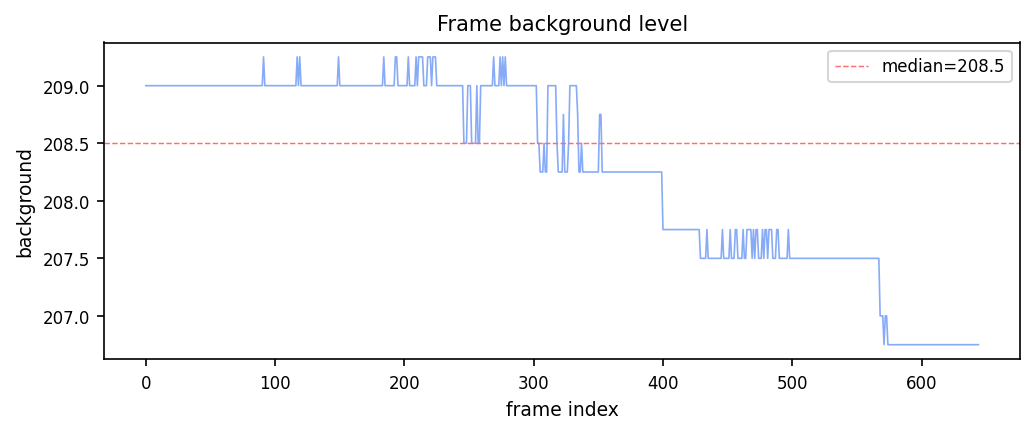
\includegraphics[width=\linewidth]{global_background.png}
    \caption{Global background trajectory.}
  \end{subfigure}
  \hfill
  \begin{subfigure}[t]{0.31\textwidth}
    \centering
    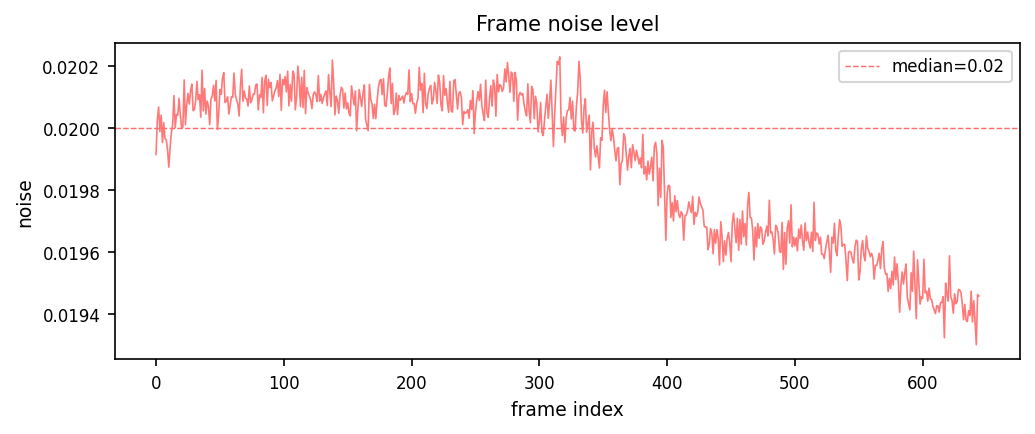
\includegraphics[width=\linewidth]{global_noise.png}
    \caption{Global noise trajectory.}
  \end{subfigure}
  \hfill
  \begin{subfigure}[t]{0.31\textwidth}
    \centering
    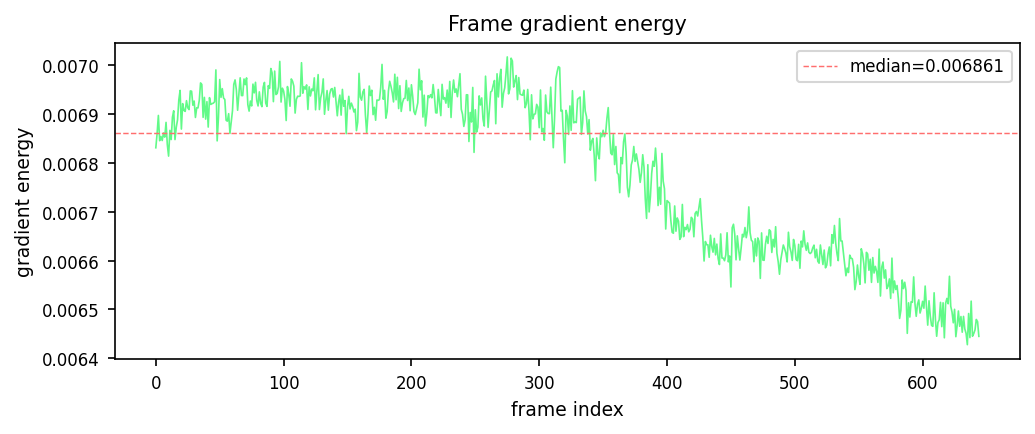
\includegraphics[width=\linewidth]{global_gradient.png}
    \caption{Global gradient-energy trajectory.}
  \end{subfigure}

  \vspace{0.45em}

  \begin{subfigure}[t]{0.31\textwidth}
    \centering
    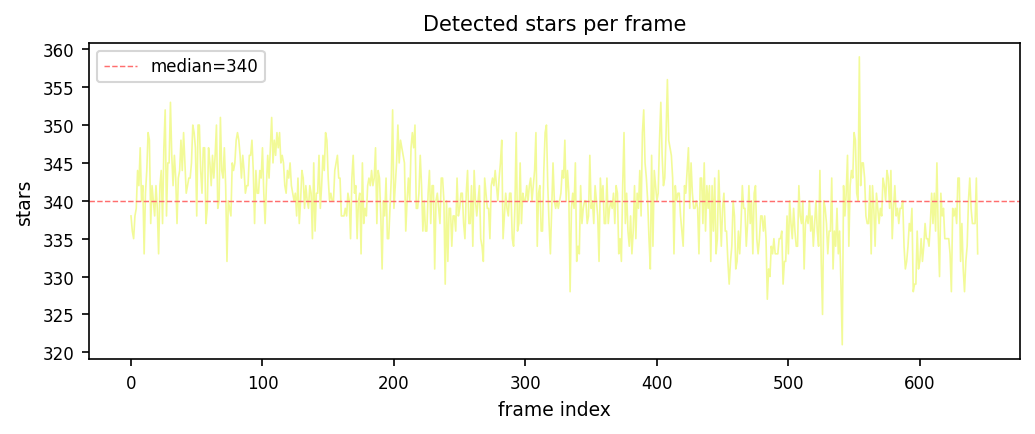
\includegraphics[width=\linewidth]{global_star_count.png}
    \caption{Detected star count per frame.}
  \end{subfigure}
  \hfill
  \begin{subfigure}[t]{0.31\textwidth}
    \centering
    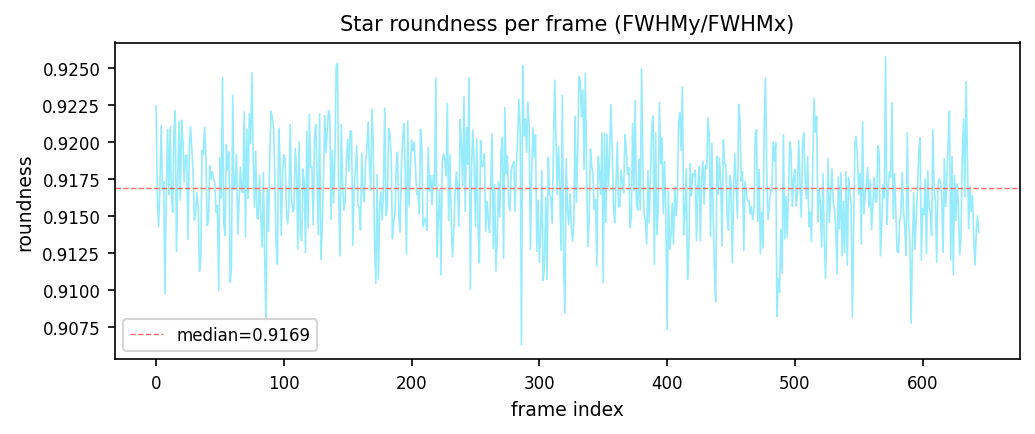
\includegraphics[width=\linewidth]{global_roundness.png}
    \caption{Global roundness trend.}
  \end{subfigure}
  \hfill
  \begin{subfigure}[t]{0.31\textwidth}
    \centering
    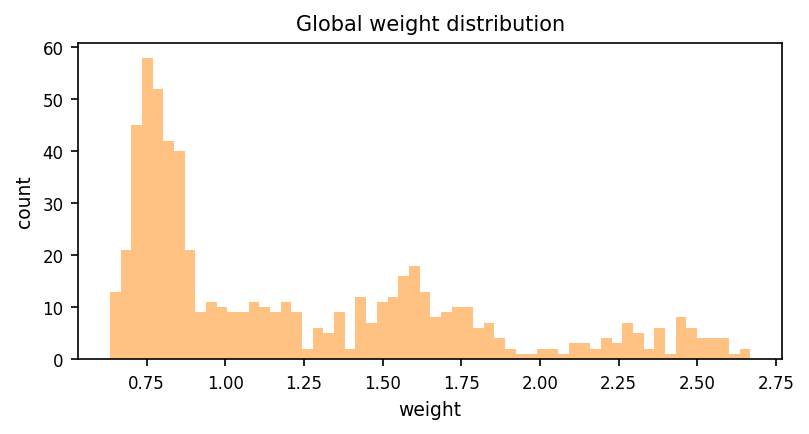
\includegraphics[width=\linewidth]{global_weight_hist.png}
    \caption{Histogram of global reconstruction weights.}
  \end{subfigure}

  \vspace{0.45em}

  \begin{subfigure}[t]{0.31\textwidth}
    \centering
    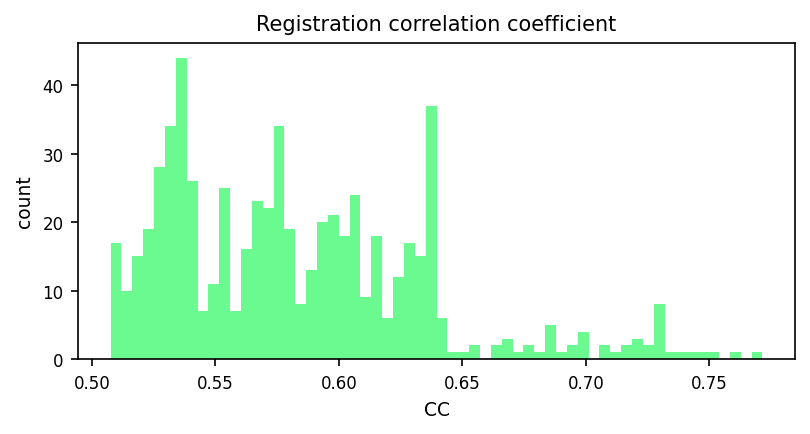
\includegraphics[width=\linewidth]{registration_cc_hist.png}
    \caption{Registration cross-correlation histogram.}
  \end{subfigure}
  \hfill
  \begin{subfigure}[t]{0.31\textwidth}
    \centering
    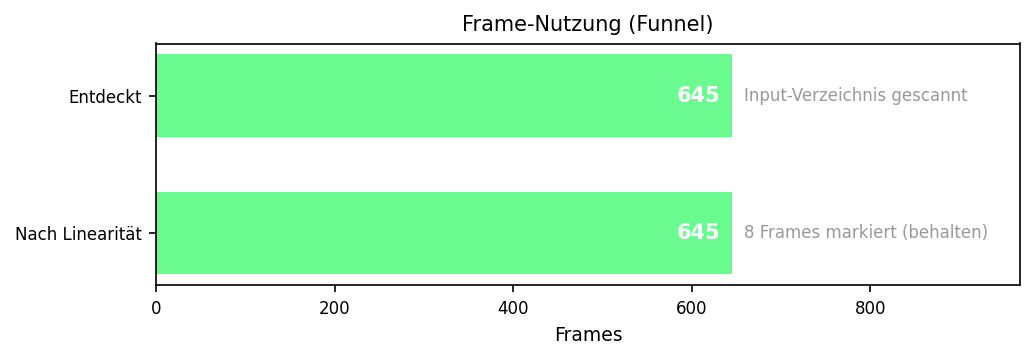
\includegraphics[width=\linewidth]{frame_usage_funnel.png}
    \caption{Frame usage funnel through the pipeline.}
  \end{subfigure}
  \hfill
  \begin{subfigure}[t]{0.31\textwidth}
    \centering
    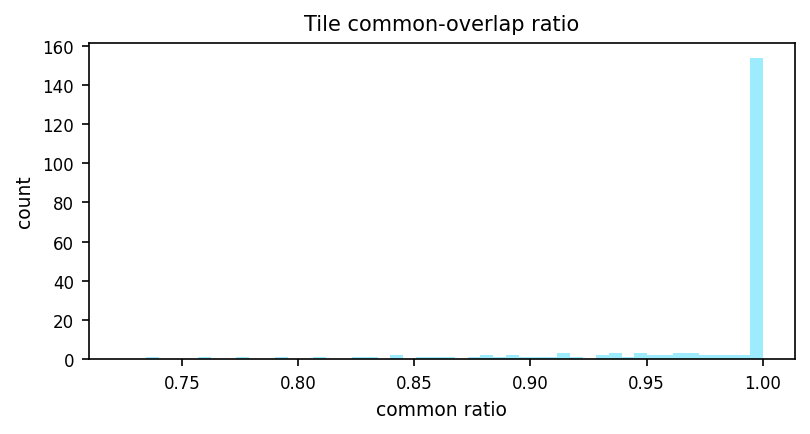
\includegraphics[width=\linewidth]{common_overlap_ratio_hist.png}
    \caption{Common-overlap ratio histogram.}
  \end{subfigure}

  \caption{Compact statistical overview for the M31 v3.3.9 run. The nine panels summarize
           frame-wise background, noise, gradient energy, source detectability, roundness,
           overlap stability, global weight distribution, registration correlation, and
           frame-flow behavior.}
  \label{fig:stats_overview}
\end{figure*}

\noindent
State-clustering diagnostics show that the dataset separates into 12 synthetic atmospheric
states. Cluster sizes range from 25 to 101 frames with a median of approximately 51 frames,
which is sufficient to support tile-weighted synthetic-frame formation. The mass-preserving
aggregation (v3.3.9) ensures that the large cluster ($|k|=101$) exerts mass-proportional
influence in the final stack rather than being over- or under-weighted by quality alone.

\begin{figure*}[!t]
  \centering
  \begin{subfigure}[t]{0.31\textwidth}
    \centering
    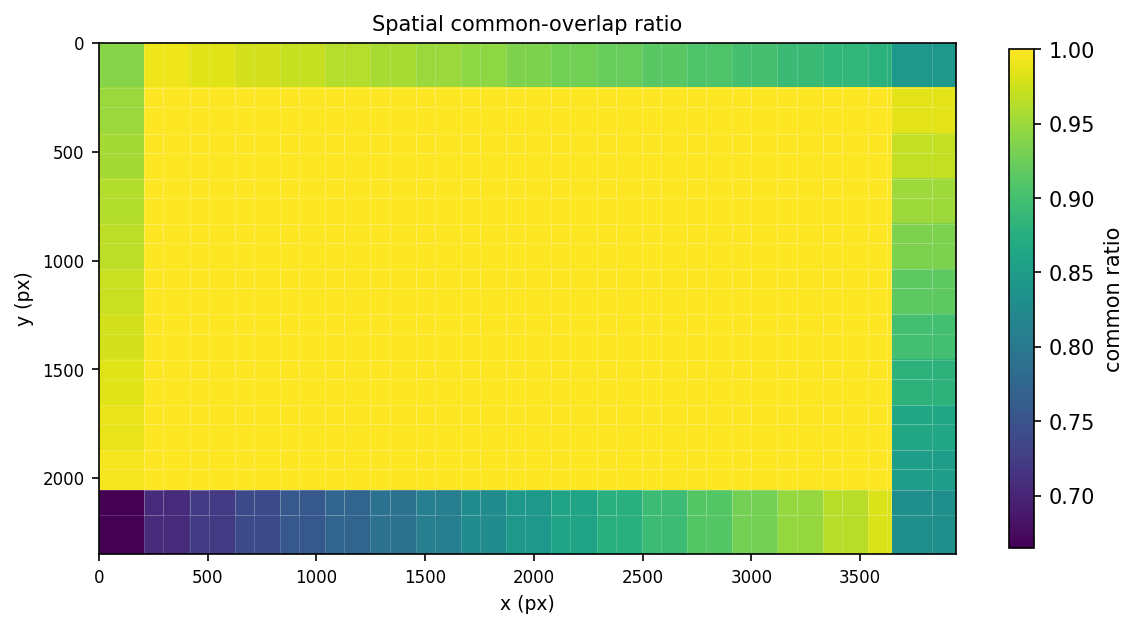
\includegraphics[width=\linewidth]{art_common_overlap_ratio_spatial.png}
    \caption{Spatial map of common-overlap ratio.}
  \end{subfigure}
  \hfill
  \begin{subfigure}[t]{0.31\textwidth}
    \centering
    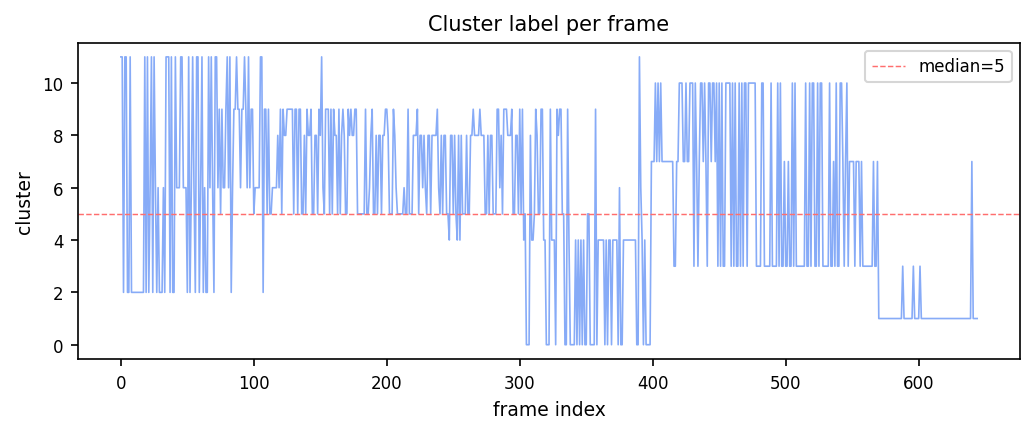
\includegraphics[width=\linewidth]{art_clustering_labels.png}
    \caption{Temporal clustering labels across the frame sequence.}
  \end{subfigure}
  \hfill
  \begin{subfigure}[t]{0.31\textwidth}
    \centering
    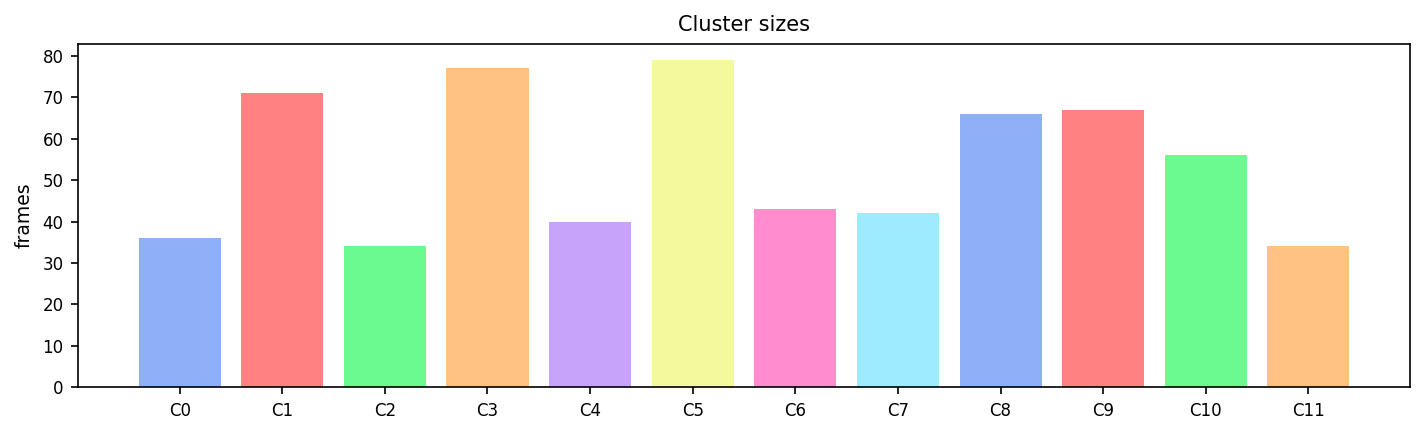
\includegraphics[width=\linewidth]{art_clustering_sizes.png}
    \caption{Cluster-size distribution for the synthetic states.}
  \end{subfigure}

  \vspace{0.45em}

  \begin{subfigure}[t]{0.31\textwidth}
    \centering
    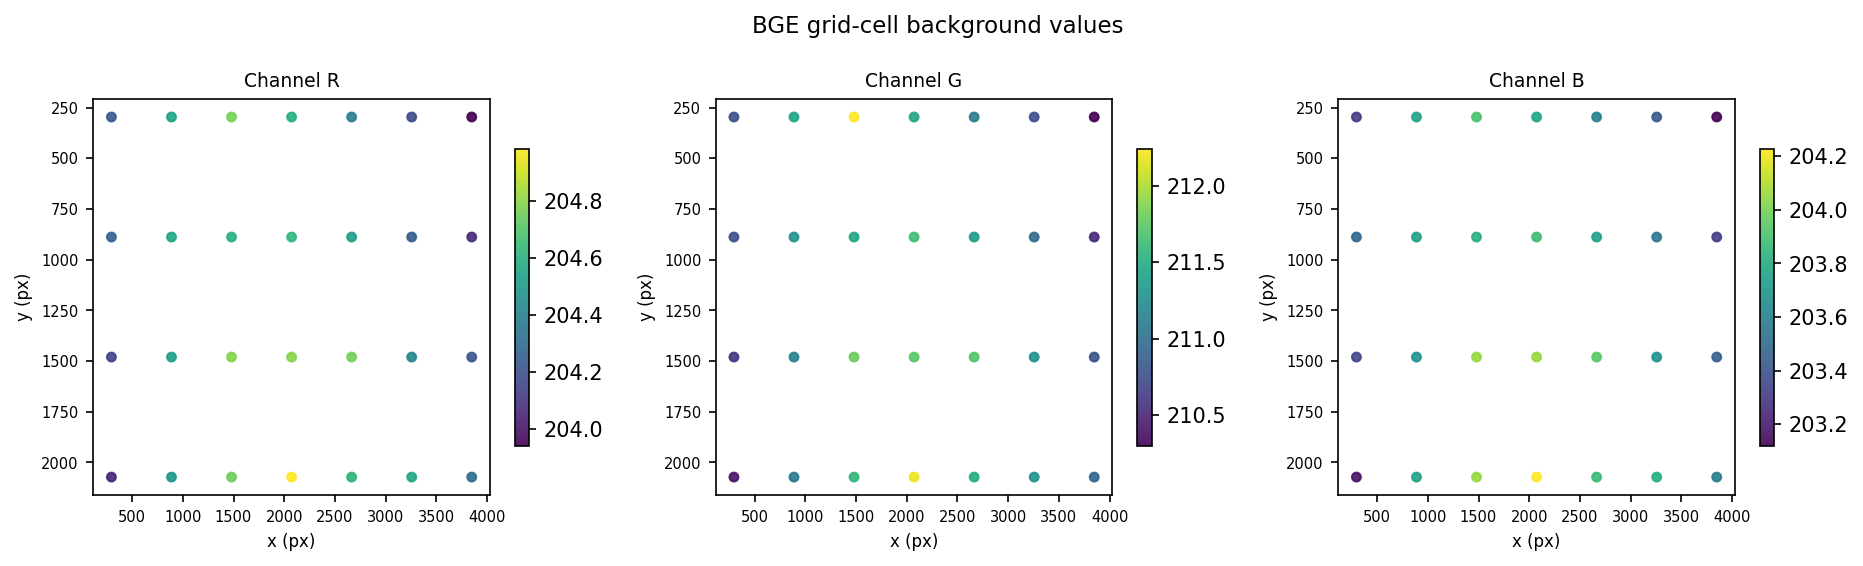
\includegraphics[width=\linewidth]{art_bge_grid_cells.png}
    \caption{BGE coarse-grid cells used for surface fitting.}
  \end{subfigure}
  \hfill
  \begin{subfigure}[t]{0.31\textwidth}
    \centering
    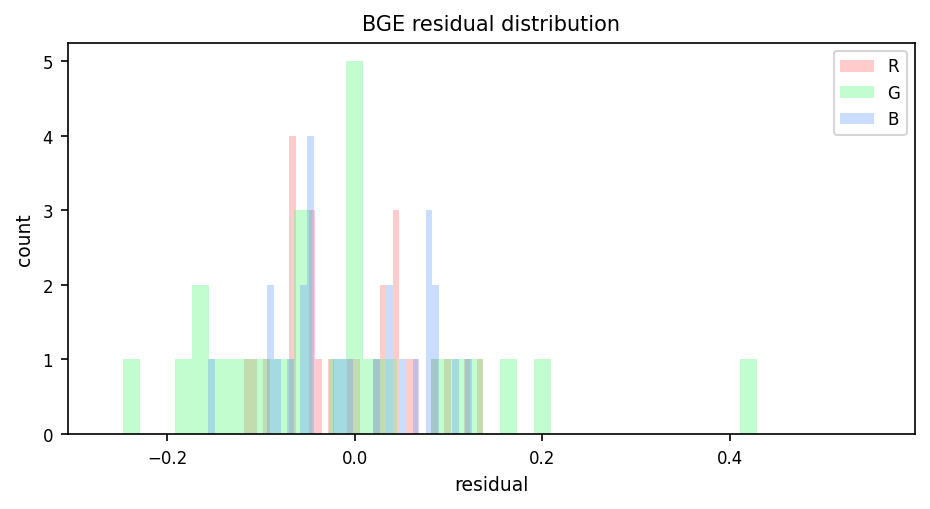
\includegraphics[width=\linewidth]{art_bge_residual_hist.png}
    \caption{Residual histogram of the fitted BGE surface.}
  \end{subfigure}
  \hfill
  \begin{subfigure}[t]{0.31\textwidth}
    \centering
    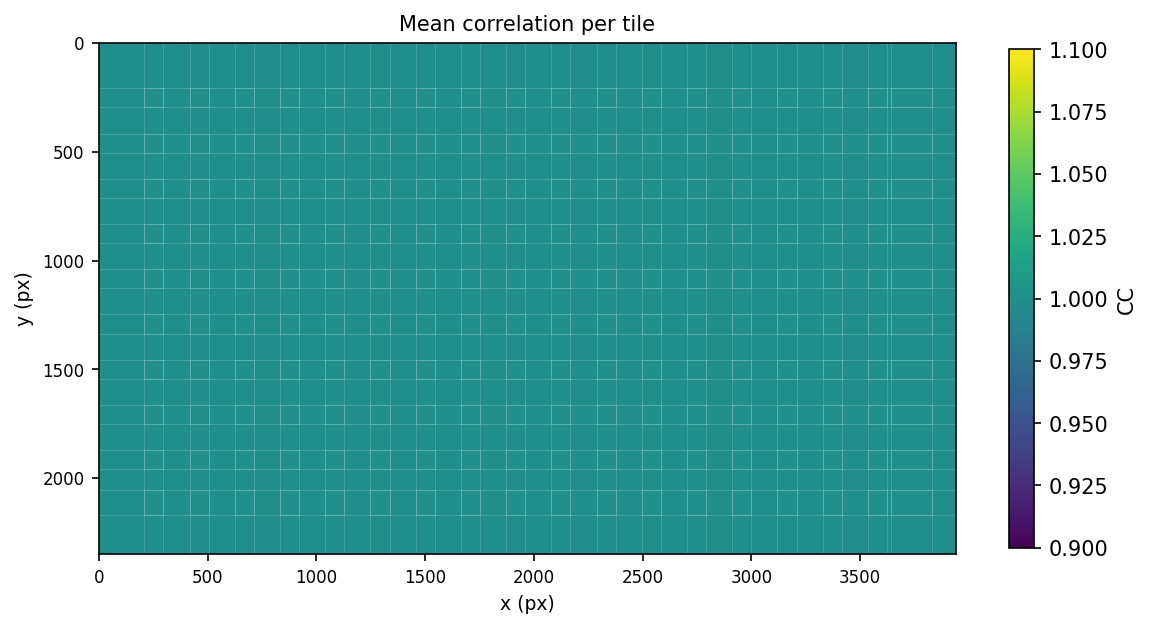
\includegraphics[width=\linewidth]{art_recon_cc_spatial.png}
    \caption{Spatial correlation structure of reconstructed tiles.}
  \end{subfigure}

  \vspace{0.45em}

  \begin{subfigure}[t]{0.48\textwidth}
    \centering
    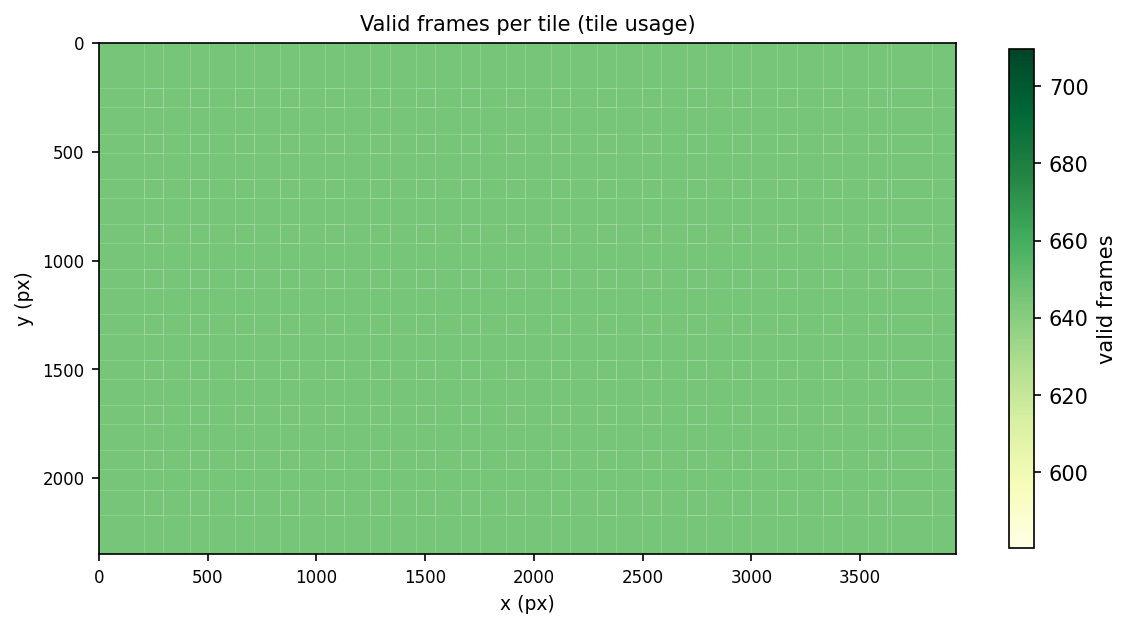
\includegraphics[width=\linewidth]{art_recon_valid_counts_spatial.png}
    \caption{Spatial distribution of valid frame counts contributing to reconstruction.}
  \end{subfigure}

  \caption{Technical diagnostics from the v3.3.9 example run. The overlap maps characterize
           geometric support, the clustering plots show how the temporal state model partitions
           the sequence into 12 atmospheric states, and the BGE/reconstruction diagnostics
           confirm that the extended-strategy RBF fit (cv RMS \num{0.0896}, normalized
           objective $J=\num{0.000440}$) and support-aware OLA produce spatially stable
           background modeling and tile-wise reconstruction coverage.}
  \label{fig:art_generated_diagnostics}
\end{figure*}

\noindent
The reconstruction-side diagnostics are consistent with the validation summary.
No tile fallback is triggered in any of the 209 tiles. Tile weight variance is \num{2.586}
and the measured FWHM improvement is \num{58.640}\% from a median seeing of \num{12.351}~px
to a median output FWHM of \num{5.108}~px. These diagnostics confirm that the v3.3.9
reformulation maintains coherent overlap support, state partitioning, additive background
modeling, and local reconstruction coverage on a real deep-sky dataset.

\end{document}
